% Interview Tutor: architecture and design review
% Repository snapshot: 4 October 2026. No credentials belong in this source.
% Build from the project root, twice:
%   pdflatex -interaction=nonstopmode -halt-on-error -output-directory=docs/presentations docs/presentations/architecture-design.tex
% Beamer notes are hidden in the presentation PDF and editable below.
\documentclass[aspectratio=169,11pt]{beamer}
\usepackage[T1]{fontenc}
\usepackage{lmodern}
\usepackage{booktabs,tabularx,array}
\usepackage{tikz}
\usepackage{listings}
\usetikzlibrary{arrows.meta,positioning,fit,calc}
\usefonttheme{professionalfonts}
\renewcommand{\familydefault}{\sfdefault}
\definecolor{Navy}{HTML}{17324D}
\definecolor{Teal}{HTML}{007E87}
\definecolor{Slate}{HTML}{4D5D6C}
\definecolor{Mist}{HTML}{EEF3F6}
\definecolor{Rule}{HTML}{CBD5DF}
\definecolor{Amber}{HTML}{A46513}
\setbeamercolor{normal text}{fg=Navy,bg=white}
\setbeamercolor{structure}{fg=Teal}
\setbeamercolor{frametitle}{fg=Navy}
\setbeamercolor{alerted text}{fg=Amber}
\setbeamercolor{itemize item}{fg=Teal}
\setbeamercolor{itemize subitem}{fg=Teal}
\setbeamerfont{frametitle}{size=\Large,series=\bfseries}
\setbeamertemplate{navigation symbols}{}
\setbeamertemplate{itemize item}{\small\raise1pt\hbox{\textbullet}}
\setbeamersize{text margin left=9mm,text margin right=9mm}
\setbeamertemplate{footline}{%
  \leavevmode\hbox{%
    \begin{beamercolorbox}[wd=.83\paperwidth,ht=3.7mm,dp=1.5mm,leftskip=9mm]{normal text}
      \fontsize{7}{8}\selectfont\color{Slate}Interview Tutor \enspace|\enspace Architecture and design
    \end{beamercolorbox}%
    \begin{beamercolorbox}[wd=.17\paperwidth,ht=3.7mm,dp=1.5mm,rightskip=9mm plus1fil]{normal text}
      \hfill\fontsize{7}{8}\selectfont\color{Slate}\insertframenumber\,/\,\inserttotalframenumber
    \end{beamercolorbox}}}
\setbeameroption{hide notes}
\hypersetup{pdftitle={Interview Tutor - Architecture and Design Review},
  pdfauthor={Project design review},pdfsubject={Implemented architecture and design, 4 October 2026},
  colorlinks=true,urlcolor=Teal,linkcolor=Navy}
\newcommand{\code}[1]{\texttt{\detokenize{#1}}}
\newcommand{\source}[1]{\par\vfill{\raggedright\fontsize{7}{8.5}\selectfont\color{Slate}Source: #1\par}}
\newcommand{\lead}[1]{{\large\color{Teal}#1\par}\vspace{3mm}}
\newcommand{\gap}{\vspace{3mm}}
\newcolumntype{Y}{>{\raggedright\arraybackslash}X}
\newcolumntype{L}[1]{>{\raggedright\arraybackslash}p{#1}}
\lstset{basicstyle=\ttfamily\fontsize{9}{11}\selectfont,
  keywordstyle=\color{Teal}\bfseries,commentstyle=\color{Slate},
  stringstyle=\color{Amber},backgroundcolor=\color{Mist},
  frame=none,xleftmargin=2mm,xrightmargin=2mm,
  columns=fullflexible,keepspaces=true,showstringspaces=false,
  breaklines=true,aboveskip=3mm,belowskip=2mm}
\tikzset{
  component/.style={draw=Navy,fill=Mist,rounded corners=1mm,
    text width=2.6cm,align=center,minimum height=9mm,inner sep=3mm,font=\small},
  external/.style={component,fill=white,draw=Teal},
  smallcomponent/.style={component,text width=2.3cm,font=\fontsize{9.5}{11}\selectfont},
  edge/.style={-{Stealth[length=2mm]},thick,draw=Navy},
  returned/.style={edge,dashed,draw=Teal},
  annotation/.style={font=\fontsize{8.5}{10}\selectfont,text=Slate,fill=white,inner sep=1mm},
  boundary/.style={draw=Rule,dashed,rounded corners=1mm,inner sep=4mm},
  lifeline/.style={draw=Rule,dashed},
}
\title{Interview Tutor}
\subtitle{Architecture and design review}
\date{4 October 2026}

\begin{document}

% 01
\begin{frame}[plain]
  \vspace{12mm}
  {\Huge\bfseries Interview Tutor\par}
  \vspace{5mm}
  {\LARGE\color{Teal}Architecture and design review\par}
  \vspace{10mm}
  {\large A local Python harness for interview practice\par}
  \vspace{4mm}
  {\color{Slate}Implemented system \enspace|\enspace 4 October 2026\par}
  \note{This review describes the current repository, rather than the original larger coding-tutor proposal. The audience is a technical project reviewer. Architecture explains the boundaries; design explains the contracts and transitions inside those boundaries.}
\end{frame}

% 02
\begin{frame}[t]{System intent and scope}
  \lead{Turn a supplied page or topic into practice, feedback, and revision notes}
  \begin{columns}[T,onlytextwidth]
    \begin{column}{.49\textwidth}
      \textbf{Implemented}
      \begin{itemize}
        \item One local user and one source/topic per session
        \item Level and optional company/tier preference
        \item One question at a time, then evidence-based marks
        \item Coding or theory notes and a downloadable PDF
      \end{itemize}
    \end{column}
    \begin{column}{.46\textwidth}
      \textbf{Deferred / excluded}
      \begin{itemize}
        \item Code execution and automatic repair
        \item Adaptive questions after each answer
        \item Saved history, accounts, and billing
        \item Autonomous browsing and deployment
      \end{itemize}
    \end{column}
  \end{columns}
  \gap
  Company context influences practice; marks are not a hiring-readiness prediction.
  \source{\code{docs/requirements.md}; \code{README.md}}
  \note{The project deliberately stays small. A reference algorithm in the report is educational material, not a tested implementation. Missing enterprise services are conscious scope choices, not components that should be invented in the diagram.}
\end{frame}

% 03
\begin{frame}[t]{Requirements that drive the architecture}
  \renewcommand{\arraystretch}{1.17}
  \small
  \begin{tabularx}{\textwidth}{L{2.2cm}YY}
    \toprule
    \textbf{Requirement} & \textbf{Design response} & \textbf{Review evidence}\\
    \midrule
    SCOPE-008 & Explicit Python orchestration & \code{TutorSession} owns the loop\\
    FR-038 & Fixed plan; bounded completion & No per-answer model calls; finalization once\\
    FR-039 & Restrict source retrieval & Public address checks, bounded text, paste fallback\\
    FR-040 & Optional fresh context & Model requests; harness executes one bounded search\\
    FR-037 & Evidence-based marks & Fixed rubric, exact learner quotes, local total\\
    BUD-005/006 & Bound and account for spending & Reservations, counters, known/unknown usage\\
    FR-041 & Actionable safe failures & Fixed error categories; retain usage before parsing\\
    \bottomrule
  \end{tabularx}
  \source{\code{docs/requirements.md}; mapped checks in \code{tests/}}
  \note{A real design review traces a decision back to a requirement and then to evidence. These IDs already exist in the project. They are references, not claims that every requirement is fully verified by a live system.}
\end{frame}

% 04
\begin{frame}[t]{System context and runtime boundary}
  \centering
  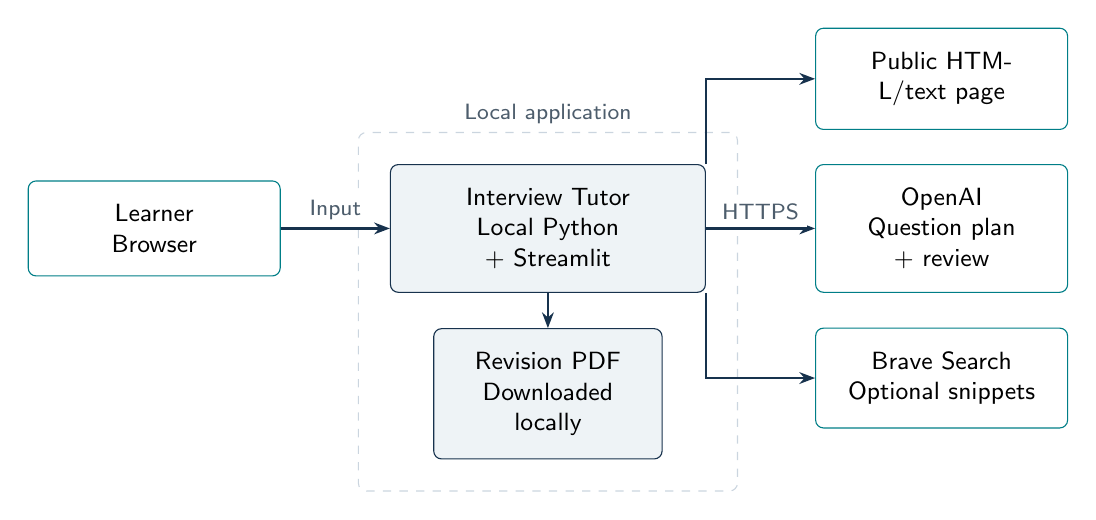
\begin{tikzpicture}
    \node[external] (user) at (0,0) {Learner\\Browser};
    \node[component,text width=3.4cm,minimum height=1.3cm] (app) at (5,0) {Interview Tutor\\Local Python + Streamlit};
    \node[external] (web) at (10,1.9) {Public HTML/text page};
    \node[external] (openai) at (10,0) {OpenAI\\Question plan + review};
    \node[external] (brave) at (10,-1.9) {Brave Search\\Optional snippets};
    \node[smallcomponent] (pdf) at (5,-2.1) {Revision PDF\\Downloaded locally};
    \node[boundary,fit=(app)(pdf)] (local) {};
    \node[annotation,anchor=south] at (local.north) {Local application};
    \draw[edge] (user) -- node[annotation,above]{Input} (app);
    \draw[edge] (app.north east) |- (web.west);
    \draw[edge] (app) -- node[annotation,above]{HTTPS} (openai);
    \draw[edge] (app.south east) |- (brave.west);
    \draw[edge] (app) -- (pdf);
  \end{tikzpicture}\par
  \gap
  \raggedright
  One application process; no database, worker queue, or execution sandbox.
  \source{\code{app.py}; \code{tutor/sources.py}; \code{tutor/openai_model.py}; \code{tutor/search.py}}
  \note{The browser is the UI surface of Streamlit, not a separately implemented frontend. Public pages support HTTP as well as HTTPS; the HTTPS label refers to provider connections. Clicking Start uses the configured inexpensive OpenAI model and session budget. Source material and final-review answers leave the machine for that provider; bounded research runs automatically only when requested by the model and permitted by configuration.}
\end{frame}

% 05
\begin{frame}[t]{Component responsibilities}
  \small\renewcommand{\arraystretch}{1.18}
  \begin{tabularx}{\textwidth}{L{4.2cm}Y}
    \toprule
    \textbf{Module} & \textbf{Owns}\\
    \midrule
    \code{app.py} & Input validation, Start, Streamlit session, cached PDF bytes\\
    \code{tutor/harness.py} & Workflow, budgets, state, answers, review validation\\
    \code{tutor/schemas.py} & Typed contracts, rubric, semantic validators, safe errors\\
    \code{tutor/sources.py} & Topic/paste normalization and public-page retrieval\\
    \code{tutor/openai_model.py} & Structured OpenAI responses and safe failure handling\\
    \code{tutor/search.py} & Bounded Brave query and source provenance\\
    \code{tutor/pdf_export.py} & Local document layout from existing notes\\
    \code{config.py} / \code{secrets.py} & Limits and prices / provider-specific runtime keys\\
    \bottomrule
  \end{tabularx}
  \source{Files under \code{tutor/}; \code{app.py}}
  \note{The app validates input before loading the OpenAI key and constructing the model client. Start is enabled without a separate spending checkbox. The orchestrator receives its model and optional search client rather than building them itself. That small dependency-injection seam allows deterministic tests without a framework. All modules still run in the same Python process.}
\end{frame}

% 06
\begin{frame}[t]{End-to-end data flow}
  \vspace{3mm}
  \centering
  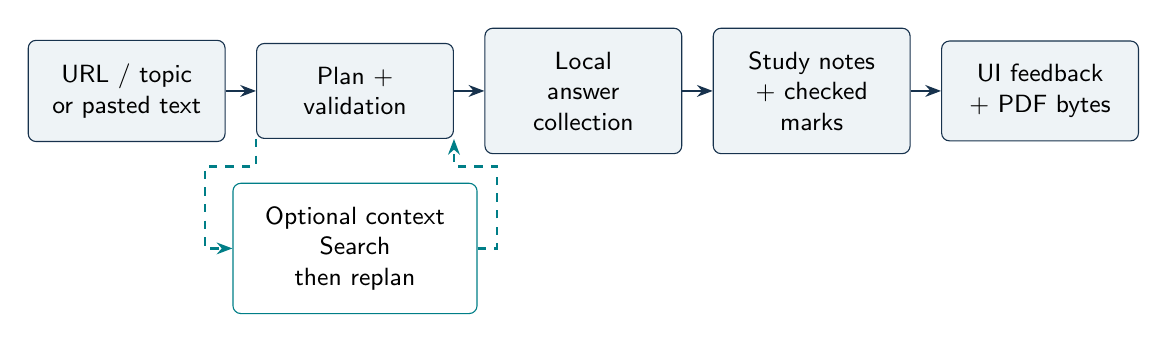
\begin{tikzpicture}
    \node[smallcomponent,text width=1.9cm] (source) at (0,0) {URL / topic\\or pasted text};
    \node[smallcomponent,text width=1.9cm] (plan) at (2.9,0) {Plan +\\validation};
    \node[smallcomponent,text width=1.9cm] (answers) at (5.8,0) {Local\\answer collection};
    \node[smallcomponent,text width=1.9cm] (review) at (8.7,0) {Study notes\\+ checked marks};
    \node[smallcomponent,text width=1.9cm] (pdf) at (11.6,0) {UI feedback\\+ PDF bytes};
    \draw[edge] (source) -- (plan);
    \draw[edge] (plan) -- (answers);
    \draw[edge] (answers) -- (review);
    \draw[edge] (review) -- (pdf);
    \node[external,text width=2.5cm] (search) at (2.9,-2) {Optional context\\Search then replan};
    \coordinate (searchin) at ([xshift=-3.5mm]search.west);
    \draw[returned] (plan.south west) -- ++(0,-.35) -| (searchin) -- (search.west);
    \draw[returned] (search.east) -- ++(.25,0) |- ([yshift=-3.5mm]plan.south east) -- (plan.south east);
  \end{tikzpicture}\par
  \gap\raggedright
  \begin{itemize}
    \item Normally: one model plan and one final model review
    \item Research adds one search and one replanning call
    \item Each answer is saved locally; PDF rendering makes no model call
  \end{itemize}
  \source{\code{TutorSession.start/send/finish}; \code{app.py}; \code{build_pdf}}
  \note{The research branch is part of planning. It is not a general browsing agent, and it is not triggered during answer collection. A download reuses the existing final review and cached bytes.}
\end{frame}

% 07
\begin{frame}[t]{Source retrieval design}
  \lead{Normalize material before the harness asks the model}
  \begin{columns}[T,onlytextwidth]
    \begin{column}{.5\textwidth}
      \textbf{Selection rules}
      \begin{itemize}
        \item Pasted text replaces URL fetching
        \item A topic can stand alone or focus a page
        \item One HTML/text page; no link traversal
        \item Retain an excerpt and label truncation
      \end{itemize}
    \end{column}
    \begin{column}{.46\textwidth}
      \textbf{Network gates}
      \begin{itemize}
        \item HTTP/S and standard ports only
        \item Reject credentials and private addresses
        \item Pin a checked IP; verify HTTPS hostname
        \item Recheck redirects and bound the response
      \end{itemize}
    \end{column}
  \end{columns}
  \gap
  Login, JavaScript, and unsupported pages need pasted material.\\
  The socket/body timeout is not a strict overall deadline.
  \source{\code{tutor/sources.py}; source integration checks in \code{tests/test_sources.py}}
  \note{Public-IP pinning helps prevent a DNS-rebinding change between validation and connection. Redirects receive the same checks. DNS and slow response headers can exceed the nominal timeout, so the deck does not promise a strict total wall-clock bound.}
\end{frame}

% 08
\begin{frame}[t]{Conditional research sequence}
  \centering
  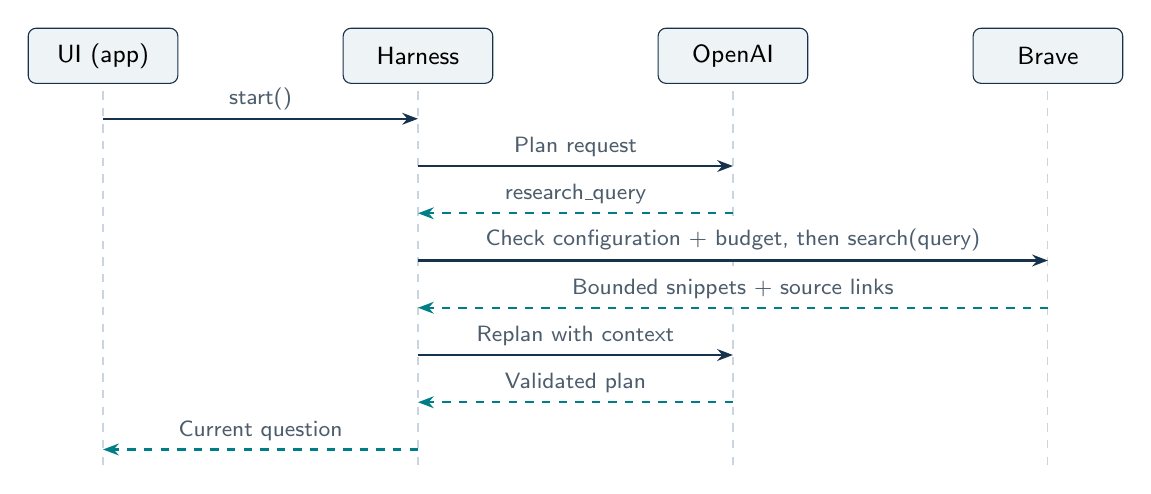
\begin{tikzpicture}[x=1cm,y=1cm]
    \foreach \name/\x/\participantTitle in {ui/0/UI (app),h/4/Harness,o/8/OpenAI,b/12/Brave}{
      \node[smallcomponent,text width=1.6cm,minimum height=7mm,inner sep=1.5mm] (\name) at (\x,0) {\participantTitle};
      \draw[lifeline] (\x,-.45) -- (\x,-5.2);
    }
    \draw[edge] (0,-.8) -- node[annotation,above]{start()} (4,-.8);
    \draw[edge] (4,-1.4) -- node[annotation,above]{Plan request} (8,-1.4);
    \draw[returned] (8,-2) -- node[annotation,above]{research\_query} (4,-2);
    \draw[edge] (4,-2.6) -- node[annotation,above]{Check configuration + budget, then search(query)} (12,-2.6);
    \draw[returned] (12,-3.2) -- node[annotation,above]{Bounded snippets + source links} (4,-3.2);
    \draw[edge] (4,-3.8) -- node[annotation,above]{Replan with context} (8,-3.8);
    \draw[returned] (8,-4.4) -- node[annotation,above]{Validated plan} (4,-4.4);
    \draw[returned] (4,-5) -- node[annotation,above]{Current question} (0,-5);
  \end{tikzpicture}
  \source{\code{tutor/harness.py}: \code{start}, \code{_research}; \code{tutor/search.py}}
  \note{This is the successful research path. A familiar stable topic can return a plan directly. There is no UI toggle: max_search_calls=0 disables research in configuration. Otherwise the harness acts on a focused model request after its budget checks. Disabled search, insufficient budget, search failure, or a repeated research request terminates planning with a partial export and a request for better source material. Result pages are not opened.}
\end{frame}

% 09
\begin{frame}[t]{Session data model}
  \lead{Runtime state is a Python object, not a persistent run database}
  \small\renewcommand{\arraystretch}{1.24}
  \begin{tabularx}{\textwidth}{L{3.3cm}Y}
    \toprule
    \textbf{Record} & \textbf{Fields retained in memory}\\
    \midrule
    Source and settings & Material, title, URL, level, company context, configuration\\
    \code{InterviewPlan} & Summary, categorized questions, optional research request\\
    Learner interaction & Raw answers and the question/answer transcript\\
    Research provenance & Query, bounded snippet context, source titles and URLs\\
    \code{StudyNotes} & Concepts, approaches, feedback, follow-ups, nullable assessment\\
    Usage and status & Attempt counts, reported tokens, estimated cost, uncertainty, notice\\
    UI artifact cache & Generated PDF bytes in Streamlit session state\\
    \bottomrule
  \end{tabularx}
  \source{\code{TutorSession.__init__}; \code{tutor/schemas.py}; \code{app.py}}
  \note{New session clears the session and PDF cache. A process restart or lost browser session can lose history. There is no durable interaction log, elapsed-time tracking, database schema, or migration layer in this version.}
\end{frame}

% 10
\begin{frame}[t]{Model response contracts}
  \begin{columns}[T,onlytextwidth]
    \begin{column}{.48\textwidth}
      \textbf{\code{InterviewPlan}}
      \gap
      \begin{itemize}
        \item Title and summary
        \item Distinct, nonblank categorized questions
        \item Plan mode: \code{research_query=null}
        \item Research mode: query + empty questions
        \item Cover every assessment category
      \end{itemize}
    \end{column}
    \begin{column}{.48\textwidth}
      \textbf{\code{StudyNotes}}
      \gap
      \begin{itemize}
        \item Summary, assumptions, key concepts
        \item Coding approaches only when relevant
        \item Feedback and common mistakes
        \item Further-practice questions and sketches
        \item Nullable evidence-based assessment
      \end{itemize}
    \end{column}
  \end{columns}
  \gap
  Strict JSON structure at the API boundary; semantic rules checked locally with Pydantic.
  \source{\code{tutor/schemas.py}; \code{tutor/openai_model.py}: \code{_response_format}}
  \note{A valid JSON object is not necessarily a valid plan. Local validators additionally check mutual exclusion, duplicate questions, category coverage, score bounds, and evidence provenance. Null allows an explicit unassessed outcome. The API schema makes nullable fields required while still permitting null.}
\end{frame}

% 11
\begin{frame}[t]{Run state machine}
  \centering
  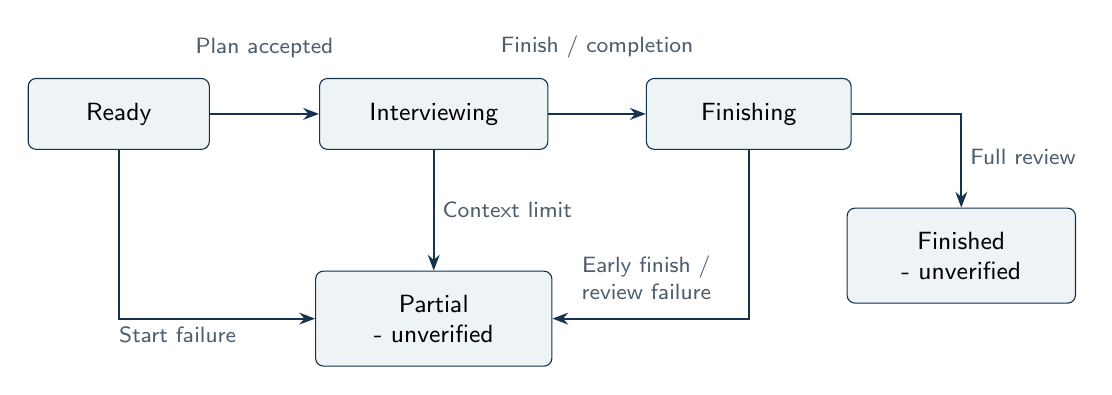
\begin{tikzpicture}
    \node[smallcomponent,text width=1.7cm] (ready) at (0,0) {Ready};
    \node[smallcomponent,text width=2.3cm] (interview) at (4,0) {Interviewing};
    \node[smallcomponent,text width=2.0cm] (finishing) at (8,0) {Finishing};
    \node[smallcomponent,text width=2.3cm] (finished) at (10.7,-1.8) {Finished\\- unverified};
    \node[smallcomponent,text width=2.4cm] (partial) at (4,-2.6) {Partial\\- unverified};
    \draw[edge] (ready) -- node[annotation,above=6mm]{Plan accepted} (interview);
    \draw[edge] (interview) -- node[annotation,above=6mm]{Finish / completion} (finishing);
    \draw[edge] (finishing.east) -| node[annotation,pos=.73,right]{Full review} (finished.north);
    \draw[edge] (ready.south) |- node[annotation,pos=.65,below]{Start failure} (partial.west);
    \draw[edge] (interview.south) -- node[annotation,right]{Context limit} (partial.north);
    \draw[edge] (finishing.south) |- (partial.east);
    \node[annotation,align=center] at (6.7,-2.08) {Early finish /\\review failure};
  \end{tikzpicture}\par
  \gap\raggedright
  Valid intermediate answers stay in \code{Interviewing}. Terminal sessions reject new answers.\\
  Planning/search happen inside \code{start()}; they are not separate stored states.
  \source{\code{tutor/harness.py}: \code{start}, \code{send}, \code{finish}}
  \note{The exact terminal strings are Finished - unverified and Partial - unverified. Even a full report remains unverified because generated code and semantic grading have not been independently proved. No-answer finish also goes directly to partial. Repeated finish calls after terminal status do nothing.}
\end{frame}

% 12
\begin{frame}[fragile,t]{Orchestration logic}
  \begin{lstlisting}[language=Python]
# Simplified pseudocode; guards remain owned by the harness.
plan = bounded_model_request(report=False)
if plan.requests_research:
    context = bounded_search(plan.query)
    plan = bounded_model_request(report=False, context=context)
    stop_partial_if_research_requested_again(plan)
accept_valid_plan(plan)

on_answer(text):
    validate_and_preserve_answer(text)   # no per-turn model call
    if report_context_over_limit: stop_partial()
    elif more_questions: show_current_question()
    else: finish_once()
\end{lstlisting}
  \gap
  The model proposes a tool request. Python authorizes, executes, validates, and stops.
  \source{\code{tutor/harness.py}: \code{_request}, \code{_research}, \code{start}, \code{send}}
  \note{This is the central harness concept: model output is a proposed next step, not permission to execute arbitrary code. Every model or tool invocation goes through bounded code paths. The snippet is explanatory pseudocode, not a replacement implementation.}
\end{frame}

% 13
\begin{frame}[t]{Final review and export sequence}
  \centering
  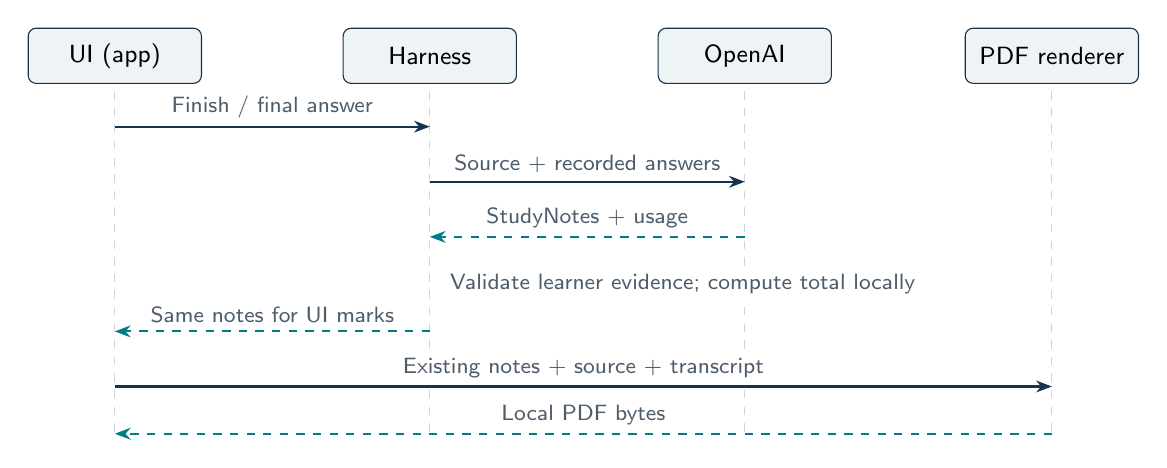
\begin{tikzpicture}
    \foreach \name/\x/\participantTitle in {ui/0/UI (app),h/4/Harness,o/8/OpenAI,p/11.9/PDF renderer}{
      \node[smallcomponent,text width=1.9cm,minimum height=7mm,inner sep=1.5mm] (\name) at (\x,0) {\participantTitle};
      \draw[lifeline] (\x,-.45) -- (\x,-4.8);
    }
    \draw[edge] (0,-.9) -- node[annotation,above]{Finish / final answer} (4,-.9);
    \draw[edge] (4,-1.6) -- node[annotation,above]{Source + recorded answers} (8,-1.6);
    \draw[returned] (8,-2.3) -- node[annotation,above]{StudyNotes + usage} (4,-2.3);
    \node[annotation,anchor=west] at (4.15,-2.9) {Validate learner evidence; compute total locally};
    \draw[returned] (4,-3.5) -- node[annotation,above]{Same notes for UI marks} (0,-3.5);
    \draw[edge] (0,-4.2) -- node[annotation,above]{Existing notes + source + transcript} (11.9,-4.2);
    \draw[returned] (11.9,-4.8) -- node[annotation,above]{Local PDF bytes} (0,-4.8);
  \end{tikzpicture}
  \source{\code{TutorSession.finish}; \code{InterviewAssessment}; \code{app.py}; \code{build_pdf}}
  \note{No answers skips the final paid review. A malformed report never produces marks. If evidence validation fails, educational notes remain available while the whole assessment is discarded. A subsequent download does not regenerate the model response.}
\end{frame}

% 14
\begin{frame}[t]{Scoring and evidence validation}
  \begin{columns}[T,onlytextwidth]
    \begin{column}{.42\textwidth}
      \small\renewcommand{\arraystretch}{1.4}
      \begin{tabularx}{\textwidth}{Yr}
        \toprule
        \textbf{Criterion} & \textbf{Marks}\\
        \midrule
        Preparation demonstrated & 3\\
        Concept knowledge & 3\\
        Scenario application & 2\\
        Reasoning and clarity & 2\\
        \midrule
        Total computed in Python & 10\\
        \bottomrule
      \end{tabularx}
    \end{column}
    \begin{column}{.53\textwidth}
      \begin{itemize}
        \item Integer marks must stay within each bound
        \item Every scored criterion needs an exact quote from one raw learner answer
        \item Missing evidence means \code{null}, not zero
        \item No total unless every criterion is assessed
        \item Invalid evidence discards the assessment
      \end{itemize}
    \end{column}
  \end{columns}
  \gap
  Provenance checks constrain the score; they do not prove that the model's judgment is correct.
  \source{\code{tutor/schemas.py}: rubric, \code{validate_marks}, \code{validate_evidence}}
  \note{A model cannot earn marks for the learner by quoting a page or its own explanation. Quotes spliced across two answers also fail. A wrong answer can receive zero with actual evidence; an absent answer is unassessed. Grading calibration against human reviewers remains future work.}
\end{frame}

% 15
\begin{frame}[t]{PDF design and consistency}
  \lead{Render the same accepted notes object that drives the feedback screen}
  \begin{columns}[T,onlytextwidth]
    \begin{column}{.49\textwidth}
      \textbf{Report content}
      \begin{itemize}
        \item Source, assumptions, and research links
        \item Scorecard with reasons and evidence
        \item Concepts, mistakes, and improvements
        \item Transcript and revision checklist
        \item Relevant follow-up questions
      \end{itemize}
    \end{column}
    \begin{column}{.47\textwidth}
      \textbf{Presentation rules}
      \begin{itemize}
        \item Coding approaches include code, dry runs, and complexity
        \item All code is labeled untested
        \item Missing final notes yield a partial report
        \item Escape text; wrap code for display
        \item Repeat table headers; number pages
      \end{itemize}
    \end{column}
  \end{columns}
  \source{\code{tutor/pdf_export.py}; \code{app.py}; PDF checks in \code{tests/test_tutor.py}}
  \note{The renderer makes no model call. Reusing one notes object reduces divergence between the screen and PDF, but prose/code correctness is still model-generated and unverified. Planned interview totals are omitted by app-owned labels; model prose is instructed to omit them too.}
\end{frame}

% 16
\begin{frame}[t]{Model adapter and failure containment}
  \lead{Inspect status and usage before attempting local JSON validation}
  \begin{enumerate}
    \item Send \code{Responses.create} with a strict Pydantic-derived schema
    \item Capture reported usage and inspect completion/refusal
    \item Validate completed JSON and enforce local semantic rules
    \item Return \code{ModelReply} or a fixed, sanitized \code{ModelRequestError}
  \end{enumerate}
  \gap
  \small\renewcommand{\arraystretch}{1.2}
  \begin{tabularx}{\textwidth}{L{4.1cm}Y}
    \toprule
    \textbf{Failure family} & \textbf{Session behavior}\\
    \midrule
    Authentication / quota / rate limit & Actionable safe notice; no automatic retry\\
    Network / timeout / model access & Stop and retain existing material\\
    Refusal / incomplete / invalid output & No fabricated review; retain known usage\\
    \bottomrule
  \end{tabularx}
  \source{\code{tutor/openai_model.py}; \code{ModelRequestError}; \code{TutorSession._record_usage}}
  \note{The earlier parse-in-SDK path could throw before the app received status and token counts. Current code retrieves the response first and parses locally. Error messages do not echo raw provider bodies, prompts, or credentials. An old generic warning cannot be diagnosed retrospectively.}
\end{frame}

% 17
\begin{frame}[t]{Budget and stopping design}
  \begin{columns}[T,onlytextwidth]
    \begin{column}{.48\textwidth}
      \textbf{Configured safeguards}
      \begin{itemize}
        \item \code{gpt-4.1-mini}; estimated session cap \$0.05
        \item 12 model-call attempts; one search attempt
        \item 40,000-byte prompt/schema allowance
        \item 1,800 plan / 3,500 report output tokens
        \item Bounded sources, context, and answers
      \end{itemize}
    \end{column}
    \begin{column}{.48\textwidth}
      \textbf{Admission and accounting}
      \begin{itemize}
        \item Reserve cost and final-review capacity first
        \item Reserve replan + report before search
        \item Count attempts before execution
        \item Replace reservations with known usage
        \item Unknown usage retains a conservative estimate
      \end{itemize}
    \end{column}
  \end{columns}
  \gap
  No automatic retries or model upgrades. Estimates are not an exact provider billing cap.
  \source{Configuration snapshot: \code{tutor/config.py}; gates in \code{tutor/harness.py}}
  \note{The byte bound is used conservatively as an input-token estimate, not as an exact tokenizer. Provider credits and project spending limits are separate from this application's budget. No prices or limits were changed to prepare this presentation. The displayed call limit is an API-attempt limit, not a promised interview length.}
\end{frame}

% 18
\begin{frame}[t]{Trust boundaries and security limits}
  \small\renewcommand{\arraystretch}{1.25}
  \begin{tabularx}{\textwidth}{L{2.8cm}YY}
    \toprule
    \textbf{Boundary} & \textbf{Implemented control} & \textbf{Remaining limitation}\\
    \midrule
    Public page & Public-address checks, pinning, redirect/size limits & HTTP may be plain text; no strict overall deadline\\
    Page/search text & JSON data and untrusted-context instructions & Prompt instructions are not a complete injection defense\\
    Provider keys & Runtime lookup, separate key returned, Git ignore & Local file is not an encrypted secrets vault\\
    Tool invocation & Fixed Brave endpoint and bounded query/results & Model decides relevance; snippets are unverified\\
    Generated code & Never executed by the application & No correctness or sandbox verification\\
    Local interface & Intended for one local user & No authentication or approved hosted deployment\\
    \bottomrule
  \end{tabularx}
  \source{\code{sources.py}; \code{search.py}; \code{secrets.py}; \code{harness.py}; \code{.gitignore}}
  \note{Keys are sent only to their provider as authentication, not as prompt or search content. The named-key loader may read the local file to select the relevant entry. store=False is a request setting, not a promise that every provider retention mechanism is disabled. Keep the deployment local unless a separate security design is completed.}
\end{frame}

% 19
\begin{frame}[t]{Verification strategy and evidence}
  \lead{Recorded baseline: 68 local tests passed on 4 October 2026}
  \small\renewcommand{\arraystretch}{1.2}
  \begin{tabularx}{\textwidth}{L{3.1cm}Y}
    \toprule
    \textbf{Test area} & \textbf{Evidence provided}\\
    \midrule
    State and contracts & Fixed planning, completion, malformed plans, idempotent finish\\
    Boundaries and tools & Mocked public fetches, redirects, Brave bounds, key separation\\
    Budgets and failures & Stop before spending; classify failures; preserve known usage\\
    Assessment & Score bounds, single-answer quotes, source text cannot earn marks\\
    UI and PDF & Start/input gates, configured research, matching marks and export\\
    SDK transport & Real SDK with mocked HTTP; no sockets or real credentials\\
    \bottomrule
  \end{tabularx}\par
  \gap
  Live provider access, question relevance, semantic grading, and search quality remain unverified.
  \source{\code{README.md}: verification record; all six modules under \code{tests/}}
  \note{Passing tests establish deterministic behavior for the scenarios tested, not objective grading quality or full correctness. All 68 local tests passed after simplifying the input page. UI checks confirm enabled Start, absence of provider/search/approval controls and introductory/model-price captions, no client construction before valid submitted input, automatic configuration-controlled research, and existing budget/scoring/export guards. All model and tool results are test-only mocks. The unchanged historical sample PDF was previously rendered and inspected. This repository has no configured deployment pipeline or persistent production telemetry.}
\end{frame}

% 20
\begin{frame}[t]{Architecture decisions and trade-offs}
  \small\renewcommand{\arraystretch}{1.23}
  \begin{tabularx}{\textwidth}{L{3.1cm}YY}
    \toprule
    \textbf{Decision} & \textbf{Reason} & \textbf{Consequence}\\
    \midrule
    Streamlit + one process & Small setup; Python throughout & UI reruns and workflow are coupled\\
    Explicit harness & Visible guards and testable transitions & More orchestration code is maintained locally\\
    Plan questions up front & Low call count and predictable cost & No answer-driven adaptive follow-ups\\
    Pydantic + strict JSON & Shared typed response contracts & Semantic validators can still reject output\\
    In-memory sessions & No database to operate & Restart/session loss can lose progress\\
    Bounded snippet research & Fresh context through snippets & Limited context; relevance is model-dependent\\
    \bottomrule
  \end{tabularx}
  \source{\code{README.md}; \code{docs/requirements.md}; implemented module boundaries}
  \note{These are the kinds of decisions an architecture review should make explicit. Separate services, a frontend build, databases, and multi-agent frameworks were excluded because this user's goal is a small hobby project. None is implied by the diagram.}
\end{frame}

% 21
\begin{frame}[t]{Operational design and known gaps}
  \begin{columns}[T,onlytextwidth]
    \begin{column}{.48\textwidth}
      \textbf{Current operation}
      \begin{itemize}
        \item Local Streamlit process and browser session
        \item Synchronous source, model, and search calls
        \item Counters and safe notices shown in the UI
        \item Reusable PDF bytes after finalization
        \item Start uses configured model and budget
      \end{itemize}
    \end{column}
    \begin{column}{.48\textwidth}
      \textbf{Gaps to review before wider use}
      \begin{itemize}
        \item No durable history or recovery
        \item No in-flight cancel control or worker queue
        \item No persistent sanitized traces or timings
        \item No human-calibrated grading benchmark
        \item No authentication or deployment plan
      \end{itemize}
    \end{column}
  \end{columns}
  \source{\code{app.py}; \code{TutorSession}; exclusions in \code{docs/requirements.md}}
  \note{The UI has an early Finish control, not a cancellation token for an in-flight provider request. Do not confuse SDK socket timeouts with a strict application-wide deadline. These gaps are review inputs rather than features implemented as part of this presentation.}
\end{frame}

% 22
\begin{frame}[t]{Review decisions for the next iteration}
  \lead{Extend the system only when a concrete practice need justifies it}
  \begin{enumerate}
    \item \textbf{Question adaptation}\\
      Decide whether answer-driven follow-ups justify more calls and a revised budget.
    \item \textbf{Grading quality}\\
      Compare feedback with human-scored examples before treating marks as calibrated.
    \item \textbf{Session recovery}\\
      Add local persistence only if saving and resuming interviews is needed.
    \item \textbf{Code verification}\\
      Require a separate sandbox/evaluation design before any execution or repair.
  \end{enumerate}
  \source{Future options; current exclusions and approval boundaries in \code{docs/requirements.md}}
  \note{These are proposed review questions, not newly approved implementation milestones. The current application remains small. A professional design review should end with explicit decisions and remaining uncertainty rather than claim production readiness.}
\end{frame}

\appendix

% 23
\begin{frame}[t]{Appendix: module interfaces}
  \small\renewcommand{\arraystretch}{1.18}
  \begin{tabularx}{\textwidth}{L{6.4cm}Y}
    \toprule
    \textbf{Interface} & \textbf{Contract}\\
    \midrule
    \code{load_source(url, topic, pasted_text, max_chars)} & Returns normalized \code{Source}\\
    \code{TutorSession(..., model, config, search_client)} & Injects model/tool dependencies\\
    \code{start() / send(text) / finish()} & Guarded state transitions\\
    \code{generate(messages, report, max_output_tokens)} & Returns \code{ModelReply}; safe failure otherwise\\
    \code{BraveSearch.search(query, max_results)} & Returns \code{SearchContext}\\
    \code{validate_evidence(answers)} & Rejects unsupported assessment quotes\\
    \code{build_pdf(..., notes, status, research_sources)} & Returns PDF bytes; no model invocation\\
    \bottomrule
  \end{tabularx}
  \source{Public functions/classes in \code{tutor/}; signatures abbreviated for readability}
  \note{Keyword-only arguments are shown without Python's star syntax for readability. The model interface is shared by convention; no formal Python Protocol is defined. The implementation receives named flags, not an opaque agent object. Interface tests replace these dependencies with deterministic models and tools.}
\end{frame}

% 24
\begin{frame}[t]{Appendix: source map and supporting references}
  \small
  \textbf{Repository evidence}
  \begin{itemize}
    \item Scope and decisions: \code{docs/requirements.md}, \code{README.md}
    \item Runtime and orchestration: \code{app.py}, \code{tutor/harness.py}
    \item Contracts and adapter: \code{schemas.py}, \code{openai_model.py}
    \item Network and credentials: \code{sources.py}, \code{search.py}, \code{secrets.py}
    \item Artifact and limits: \code{pdf_export.py}, \code{config.py}
    \item Evidence: \code{tests/}, \code{docs/sample-notes.pdf}
  \end{itemize}
  \gap
  \textbf{Official API references for further reading}
  \begin{itemize}
    \item \href{https://developers.openai.com/api/docs/guides/structured-outputs}{OpenAI: Structured Outputs}
    \item \href{https://developers.openai.com/api/docs/guides/error-codes}{OpenAI: Error codes and Python error types}
    \item \href{https://api-dashboard.search.brave.com/api-reference/web/search}{Brave: Web Search API}
  \end{itemize}
  \source{Repository snapshot: 4 October 2026. Configuration values describe this build, not a billing guarantee.}
  \note{Every architecture and design claim is grounded in the current source files. External references are supporting API reading. The sample PDF contains illustrative mock sources and marks, not a live provider result. No paid calls or credentials were needed to create this presentation.}
\end{frame}

\end{document}
